\documentclass[11pt]{article}
\usepackage[margin=1in]{geometry}
\usepackage{amsmath,amssymb,amsthm,mathtools}
\usepackage{graphicx}
\usepackage{microtype}
\usepackage[hidelinks]{hyperref}

\newtheorem{theorem}{Theorem}
\newtheorem{remark}{Remark}
\newcommand{\R}{\mathbb R}
\newcommand{\Z}{\mathbb Z}
\newcommand{\ind}{\mathbf 1}
\newcommand{\Span}{\operatorname{span}}

\title{The Nonstationary Twisted Spaces in Example 5.7 Are Not Nested\\
\large A negative answer to the printed twisted-wavelet question}
\author{Autonomous counterexample candidate for human review}
\date{11 August 2026}

\begin{document}
\maketitle

\begin{center}
\fbox{\parbox{0.91\textwidth}{\textbf{Status.}
Candidate full negative answer to the wavelet-existence question as printed,
likely valid.  The spaces in the source construction fail the first nesting
axiom of a nonstationary multiresolution analysis.  The separate conjecture on
Riesz sequences of all twisted B-splines is not resolved.}}
\end{center}

\section{Source construction and question}

Das, Massopust, and Radha \cite{DMR} define a nonstationary twisted
multiresolution analysis by requiring, in particular,
\[
  V_j\subseteq V_{j+1}\qquad(j\in\Z).
\]
In Example 5.7 (source PDF pages 26--28), they take
\[
 \phi=\phi_1=\ind_{[0,1)\times[0,1)},\qquad
 N_j=2^j\phi(2^j\,\cdot,2^j\,\cdot),\qquad \Phi_j=N_{2j},
\]
and define $V_j$ as the closed span of
\[
 g_{j,k,l}:=
 D_{2^{-j}}
 \bigl(T^{t}_{(2^{-j}k,2^{-j}l)}\bigr)^{2^{2j}}\Phi_j,
 \qquad k,l\in\Z.
\]
Here $D_af(x,y)=a f(ax,ay)$ and
\[
 \bigl(T^t_{(u,v)}\bigr)^\lambda f(x,y)
 =e^{\pi i\lambda(vx-uy)}f(x-u,y-v).
\]
The source computes
\begin{equation}\label{eq:generator}
 g_{j,k,l}(x,y)
 =2^j e^{\pi i(lx-ky)}
 \ind_{[k,k+2^{-j})\times[l,l+2^{-j})}(x,y),
\end{equation}
then infers nesting from the fact that the level-$(j+1)$ support square is
contained in the level-$j$ square.  This implication goes in the wrong
direction.

\begin{figure}[ht]
 \centering
 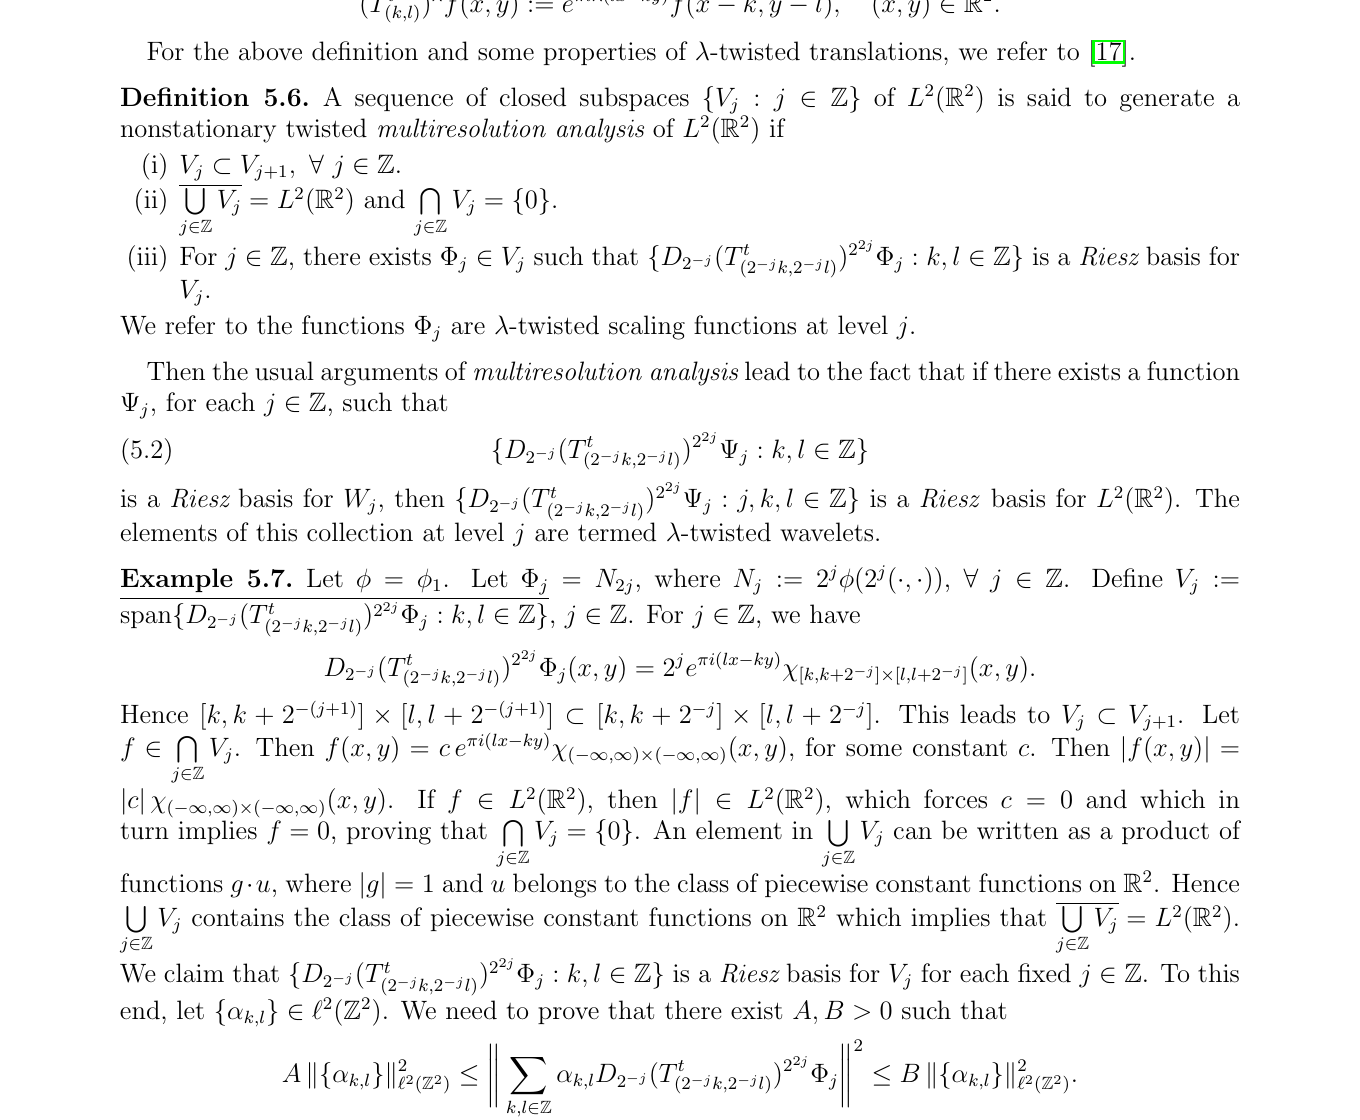
\includegraphics[width=\textwidth]{figures/construction_crop.png}
 \caption{Definition 5.6 and the construction and support formula in Example
 5.7, source PDF page 26.}
\end{figure}

At the bottom of page 28 the authors ask whether one can find $\Psi_j$ whose
twisted translates form a Riesz basis for $W_j$, where
$V_j\oplus W_j=V_{j+1}$, and thereby obtain a Riesz basis for $L^2(\R^2)$.

\begin{figure}[ht]
 \centering
 
\includegraphics[width=\textwidth]{figures/open_problem_crop.png}
 \caption{The open wavelet-existence question, source PDF page 28.}
\end{figure}

\section{Proof intuition}

At every nonnegative level the generators occupy small squares anchored at
integer lattice points.  Increasing the level makes each occupied square
smaller but does not refine the integer anchor lattice.  Thus level $j+1$
leaves open gaps inside the supports occupied at level $j$.  Closure of a span
cannot create mass outside the union of the supports of its generators.  A
single level-$j$ generator therefore witnesses the failure of nesting.

\section{Negative answer}

For $j\geq0$, set
\[
 E_j=\bigcup_{k,l\in\Z}
 [k,k+2^{-j})\times[l,l+2^{-j}).
\]

\begin{theorem}\label{thm:main}
For the spaces in Example 5.7,
\[
 V_j\not\subseteq V_{j+1}\qquad\text{for every }j\geq0.
\]
In particular there is no subspace $W_0$ with
$V_0\oplus W_0=V_1$.  Hence no family $(\Psi_j)_{j\in\Z}$ satisfying the
open question exists for the spaces as defined.
\end{theorem}

\begin{proof}
Equation~\eqref{eq:generator} shows that every level-$j$ generator is
supported in $E_j$.  Therefore every finite linear combination is supported
in $E_j$.  The subspace
\[
 L^2(E_j)=\{f\in L^2(\R^2):f=0\text{ a.e. on }\R^2\setminus E_j\}
\]
is closed, so
\begin{equation}\label{eq:support}
 V_j\subseteq L^2(E_j).
\end{equation}

Fix $j\geq0$ and take the level-$j$ generator with $k=l=0$:
\[
 g_{j,0,0}=2^j\ind_{[0,2^{-j})\times[0,2^{-j})}\in V_j.
\]
Consider the positive-measure rectangle
\[
 R_j=\bigl(2^{-(j+1)},2^{-j}\bigr)
     \times\bigl(0,2^{-(j+1)}\bigr).
\]
Because $j\geq0$, the only level-$(j+1)$ square meeting the open unit cell
$(0,1)\times(0,1)$ is
$[0,2^{-(j+1)})\times[0,2^{-(j+1)})$.  Consequently
$R_j\cap E_{j+1}=\varnothing$.  But $g_{j,0,0}=2^j$ throughout $R_j$.
It follows from \eqref{eq:support} at level $j+1$ that
$g_{j,0,0}\notin V_{j+1}$.  Hence $V_j\not\subseteq V_{j+1}$.

If $V_0\oplus W_0=V_1$ for any subspace $W_0$, then necessarily
$V_0\subseteq V_1$, contradicting the case $j=0$.  Thus the requested
$W_0$ and $\Psi_0$ do not exist, and neither can the requested all-level
family.
\end{proof}

\section{Direct algebra check and scope}

For completeness, the displayed support formula follows directly from the
source definitions.  Substitution gives
\begin{align*}
g_{j,k,l}(x,y)
 &=2^{-j}e^{\pi i2^{2j}
 ((2^{-j}l)(2^{-j}x)-(2^{-j}k)(2^{-j}y))}\\
 &\quad\times
 2^{2j}\phi\bigl(2^{2j}(2^{-j}x-2^{-j}k),
                   2^{2j}(2^{-j}y-2^{-j}l)\bigr)\\
 &=2^j e^{\pi i(lx-ky)}
 \ind_{[k,k+2^{-j})\times[l,l+2^{-j})}(x,y).
\end{align*}
Thus the counterexample does not depend on an OCR reading or a numerical
plot.

This resolves the literal existence question for Example 5.7, not every
possible corrected construction.  One could repair the support defect by
changing the scale/translation convention so that the anchor lattice refines
with the support, but that would define different spaces and a new problem.
The all-orders Riesz-sequence conjecture in Section 4 is also separate.

\section{Verification and novelty status}

The proof uses only supports and closedness of $L^2(E_j)$.  The decisive
review point is whether the published formula \eqref{eq:generator} and the
definition of $V_j$ are intended literally.  A bounded search of the run
indexes, arXiv, the 2022 journal record, and later papers citing the source
found no explicit correction or resolution of this exact wavelet question.
Priority is therefore not asserted; the mathematical status is a candidate
counterexample pending human review.

\begin{thebibliography}{9}
\bibitem{DMR}
S.~R. Das, P.~Massopust, and R.~Radha,
\emph{Twisted B-splines in the complex plane},
Appl. Comput. Harmon. Anal. 56 (2022), 250--282;
arXiv:2009.04146.
\end{thebibliography}

\end{document}
